\subsection{Sphere-geodesic-line picking}
\label{sec:sphere_geodesic_line}


nD-Sphere-geodesic-line picking is similar to sphere-line picking, except
that the ``lines'' are geodesics on the surface of the sphere, and the
distance metric is the length of these lines.

Figures ...

\begin{figure}[tbp]
  \begin{center}
    \subfloat[\label{fig:sphere_geo_eg}
    Example.]{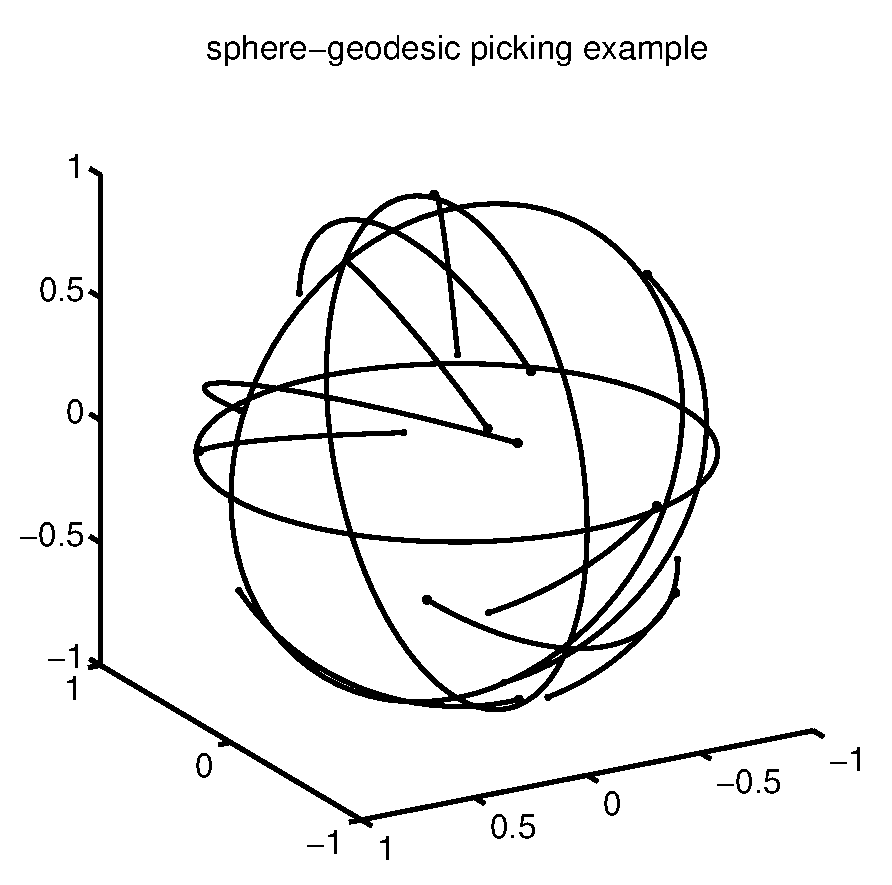
\includegraphics[width=0.4\columnwidth]{../Matlab/Plots/LinePicking_test_sim_sphere_geodesic_eg.eps}} 
    \hspace{6mm}
    \subfloat[\label{fig:sphere_geo_pdf}PDF.]{\includegraphics[width=0.48\columnwidth]{../Matlab/Plots/LinePicking_test_sim_sphere_geodesic.eps}}
    \caption{The sphere-geodesic-line picking problem.}
  \end{center} 
\vspace{-4mm}
\end{figure}

\subsubsection{PDF}

As in the $n$-Sphere above we first determine a density $f(\phi_1)$ function for $\phi_1$ then using the transform method.
\begin{equation}
g_{R}^{n}(t)=\frac{\Gamma\left(\frac{1+n}{2}\right) \sin\left(\frac{t}{R}\right)^{n-1}}{\sqrt{\pi } R \Gamma\left(\frac{n}{2}\right)}
\end{equation}

\subsubsection{CDF}
\begin{equation}
G_{R}^{n}(t)=\frac{1}{2}-\frac{\cos\left(\frac{t}{R}\right) \sin\left(\frac{t}{R}\right)^n \left(\sin\left(\frac{t}{R}\right)^2\right)^{-n/2}\Gamma\left(\frac{1+n}{2}\right) {}_{2}F_{1}\left(\frac{1}{2},1-\frac{n}{2},\frac{3}{2},\cos\left(\frac{t}{R}\right)^2\right) }  {\sqrt{\pi } \Gamma\left(\frac{n}{2}\right)}
\end{equation}

\subsubsection{Moments}

\begin{equation}
E[g_{R}^{n}(t)]=\frac{\pi R}{2}
\end{equation}



